\documentclass[a4paper, onecolumn, 10pt]{IEEEtran}

\renewcommand{\baselinestretch}{2}

\usepackage{graphicx}
\usepackage{caption}
\usepackage{hyperref}
\usepackage{setspace}
\usepackage{indentfirst}


\onehalfspacing

\begin{document}

\title{Soft and Biohybrid Robotics Project 3 Report}
\author{Matthias Heyrman}
\date{}
\maketitle

\section{Finger Controller}
\label{sec::3}

In SOFA, a simple finger controller was created using the already provided goal tracking finger. A controller was developed that, on every animation event, calculates a sinusoidal position for the finger to move at every time step as follows:
\begin{equation}
	x = pos[0] - 30 * |sin(\frac{t * 170 * \pi}{180})|,  y = pos[2] + 30 * cos(\frac{t * 170 * \pi}{180})
\end{equation}
The error metrics were tracked as the delta between the goal fingertip location and the true fingertip location and plotted using the matplotlib library, shown in Figure \ref{fig1}.
\begin{figure}[!htbp]
        \centering
        \captionsetup{justification=centering}
        \centering
        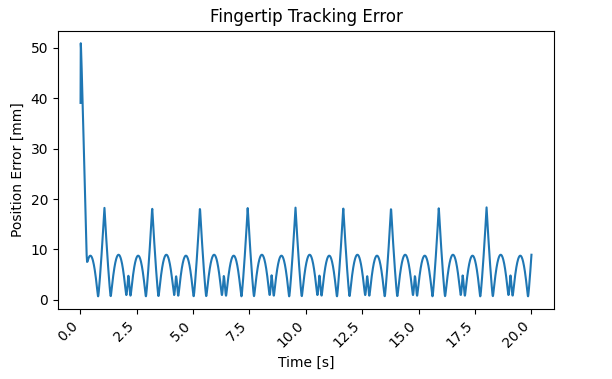
\includegraphics[width=0.45\textwidth]{Task3_error_2.png} 
        \caption{Fingertip tracking error for finger controller.}
        \label{fig1}
\end{figure}
There is a large error at the beginning of the error due to the goal position and the finger tip position not being at the same location, but the fingertip quickly moves the reach the goal. Afterwards, there is a pattern of error increasing and decreasing. This is caused by the goal location being moved in a smooth arc of radius 30mm, while the finger itself is not capable of exactly tracking this arc, as can be seen in the accompanying video.

\section{Custom Gripper}
\label{sec::4}
Based on learnings from \ref{sec::3}, a custom gripper and controller were to be made and programmed to autonomously pickup and place objects in SOFA. To accomplish this, much was based on the provided CableGripper tutorial in the SoftRobots plugin provided with SOFA. This tutorial arranges 3 fingers in a gripper formation in a fixed relative location that can then be controlled. However, as this assignment required a full gripper, instead a gripper palm was designed using SOLIDWORKS and combined with the finger meshes in Fusion 360, with an STL and VTK file being created using gmsh to be imported using SofaPython3. This cables had to oriented properly within the gripper's mesh to pull at the fingers to create a grasping motion.

A controller was written to automatically move between various states. The main states were moving towards and object, and grasping the object. Three objects were chosen from the YCB dataset, as specified in the project instructions. The provided meshes were optimized using gmsh, however, this did not seem to help the final performance much. The objects chosen had basic shapes (spherical, cylindrical, and cubic) so it was easy to calculate their inertia matrices using commonly found masses and sizes, which enables more realistic interactions within SOFA. The object positions were hardcoded into the controller, as object detection is outside the range of this project.

Once the controller's state machine was ready, the task worked automatically, and is shown in the accompanying video moving to, grasping, moving, and placing 3 imported objects. One main comment is that due to the number of interactions between meshes of the gripper and the imported objects, the software runs noticeably slower during the object handling states. This is important to note, and in the future, more care will be taken to optimize the shapes of the objects to minimize the number of collisions to calculate. The code used is provided with this assignment for inspection alongside detailed comments.

\end{document}
